\documentclass{beamer}
\usetheme{Frankfurt}

\usepackage{algpseudocodex}

\usepackage{pgfpages}
\usepackage{awesomebox}
\usepackage{amsmath}
\usepackage{amssymb}
\usepackage{comment}
\usepackage{listings}
\usepackage{booktabs}

\newcommand{\itab}{Cormen et al. Introduction to Algorithms, Third Edition (3rd. ed.). The MIT Press.}

\newcommand{\seqa}[1]{$\lang #1 \rangle$}
\newcommand{\seqb}[2]{$#1 =\langle #2 \rangle$}
\setbeamertemplate{note page}{\pagecolor{yellow!5}\insertnote}\usepackage{palatino}

\AtBeginSection[]{
  \begin{frame}
  \vfill
  \centering
  \begin{beamercolorbox}[sep=8pt,center,shadow=true,rounded=true]{title}
    \usebeamerfont{title}\insertsectionhead\par%
  \end{beamercolorbox}
  \vfill
  \end{frame}
}

%\setbeameroption{show notes on second screen=right} % Both

\title{Design and Analysis of Algorithms}

\author{Rodrigo Bonif\'{a}cio}

\begin{document}
\begin{frame}
\titlepage
\end{frame}


\section{Introduction}

\begin{frame}

  \begin{block}{Introduction to Algorithms (Cormen et al.)}
  \begin{itemize}
    \item An algorithm is any well-defined computational procedure (sequence of
    steps) that takes some set of values as input and produces some set of values
    as output. \pause

  \item An algorithm is a tool for solving a well-defined computational problem. The
    statement of the problem specifies the input/output relationship. The
    algorithm describes a specific computational procedure for achieving the
    input/output relationship.
  \end{itemize}
  \end{block}

  
  \note[item]{The input must satisfy whatever constraints imposed in the problem statement. Example:
  the binary search algorithm requires as input an ordered sequence.}
  
\end{frame}

\begin{frame}

  \begin{block}{The Art of Computer Programming - Volume I - (D. Knuth)}
    \begin{itemize}
      \item The modern meaning of algorithm is similar to that of
      a method, procedure, routine, and the like. \pause An algorithm must
      additionally include five important features\pause:

      \begin{enumerate}
       \item Finiteness
       \item Definiteness
       \item Input
       \item Output
       \item Effectiveness \pause(in terms of both time and space, for instance)  
      \end{enumerate}
   \end{itemize}   
  \end{block}  
\end{frame}

\begin{frame}{Different domains are fertile of computational problems}

  \begin{itemize}
   \item Biology (e.g., DNA sequencing)
   \item Electronic commerce (e.g., ML, cryptography)
   \item Manufacturing (optimization)
   \item Compilers (parsers, data-flow analysis, \ldots)
  \end{itemize}
  
\end{frame}

\begin{frame}{Goals of this course}
  \begin{itemize}
   \item Data Structures (graphs)
   \item Techniques for {\color{blue}algorithm design and analysis}
     \begin{itemize}
       \item divide-and-conquer
       \item dynamic programming, greedy algorithms
       \item chaotic, fixing-point algorithms, \ldots  
     \end{itemize}
   \item Hard problems (aka {\color{blue}complexity} theory) 
  \end{itemize}
\end{frame}


\begin{frame}{Example: Sorting problem}

  \begin{description}
   \item[Input] A sequence of $n$ numbers $\langle a_1, a_2, \ldots, a_n \rangle$
   \item[Output] A permutation (reordering) $\langle a'_1, a'_2, \ldots, a'_n \rangle$ of the input
     sequence, such that $a'_1 \leq a'_2 \leq \ldots \leq a'_n$
  \end{description}

  \pause
  
  \begin{block}{Problem Instance}
    Given the input sequence $\langle 31, 41, 59, 26, 41, 58\rangle$,
    a sorting algorithm returns as output the sequence: \pause
    $\langle 26, 31, 41, 41, 58, 59 \rangle$
  \end{block}


\end{frame}

\begin{frame}
  Sorting is a fundamental operation in Computer Science. \pause As such,
  we have a large number of good algorithms at our disposal. \pause

  \begin{block}{Fundamental questions}
   \begin{itemize}
   \item what is the best sorting algorithm? (analysis)
   \item is this algorithm correct? (correctness proof)
   \end{itemize}  
  \end{block}
\end{frame}


\begin{frame}{Insertion Sort}
  
  \begin{itemize}
  \item An efficient algorithm for sorting an array {\bf A} with a
    {\color{blue}small number of elements}. \pause

  \item The algorithm sorts the input numbers in place---i.e., rearranging the
    numbers within the input array {\bf A} (emphasis on the procedural style). \pause 

  \item For convenience, we will assume that the indexes of an array of size $n$ are numbered
    from $1 .. n$ in the pseudocode of the algorithms. \pause The implementation assumes
    the arrays (or lists) start in the index $0$.   
  \end{itemize}
\end{frame}

\begin{frame}
  \begin{block}{Pseudocode for Insertion Sort}
  \begin{algorithmic}
    \Procedure{InsertionSort}{A}
       \For{$j = 2, \dots, A.length$} 
         \State $key \gets A[j]$
         \State $i \gets j-1$
         \While{$i > 0\ and\ A[i] > key$}
            \State $A[i+1] \gets A[i]$
            \State $i \gets i - 1$        
         \EndWhile
         \State $A[i+1] = key$  
       \EndFor
    \EndProcedure
  \end{algorithmic}  
  \end{block}

  \pause 

  \begin{block}{Analysis}
    \begin{itemize}
      \item expected (worst-case order of growth) running time
      \item correctness proof (loop invariant) 
    \end{itemize}

    \note[item]{The running time of an algorithm on a particular input is the number
      of (machine-independent) primitive operations executed.}

    \note[item]{We should consider three aspects: initialization, maintenance, and
    termination. This follows the proof-by-induction method.}
  \end{block}

\end{frame}

\begin{frame}{Merge Sort}

    \begin{itemize}
      \item a ``divide-and-conquer'' approach for sorting.
      \item worst-case running time is much less than that of insertion sort\pause:
        \begin{itemize}
         \item insertion sort: $\mathcal{O}(n^2)$ 
         \item merge sort: $\mathcal{O}(n\log{}n)$ 
        \end{itemize}
      \item Essence of the divide-and-conquer approach: many algorithm are {\color{blue}recursive} in nature. \pause
        We can decompose the problems in three steps:
        \begin{itemize}
         \item Divide
         \item Conquer
         \item Combine  
        \end{itemize}
        \pause
      \item For the Merge Sort algorithm, the {\color{blue}Combine} step is the interest one. \pause Let's discuss
        two variants of the merge sort. 
    \end{itemize}
\end{frame}

\begin{frame}
\begin{block}{(V1) The merge function returns a new, sorted array}
\begin{scriptsize}
    \begin{algorithmic}
      \Procedure{Merge}{A,B}
%       \comment{A and B are sorted arrays}
       \State $Size \gets A.length + B.length$ 
       \State $i, j, k \gets 1$  
       \State $C \gets Array[1 .. Size]$ 

%       \comment{Iterate over the elements of A and B, and copy them in sorted order}
       \While{$i \leq A.length\ and\ j \leq B.length$}
         \If{$A[i] \leq B[j]$}
           \State $C[k] \gets A[i]$
           \State $i \gets i + 1$
         \Else
           \State $C[k] \gets B[j]$
           \State $j \gets j + 1$
         \EndIf
         \State $k \gets k + 1$  
       \EndWhile
         
%% %       \comment{Copy the remaining elements of A}  
       \For{$l = i, \ldots, A.length$}
         \State $C[k] \gets A[l]$
         \State $k \gets k + 1$
       \EndFor

%% %       \comment{Copy the remaining elements of B} 
       \For{$l = j, \ldots, B.length$}
        \State $C[k] \gets B[l]$
        \State $k \gets k + 1$
       \EndFor 
       \State {\bf return} $C$
    \EndProcedure
    \end{algorithmic}
\end{scriptsize}
\end{block}
\end{frame}

\begin{frame}{Sorting with Merge Sort}

  \begin{itemize}
    \item The sort procedure is trivial. 
  \end{itemize}

  \pause

  \begin{block}{Top-level procedure of merge sort}
    \begin{scriptsize}
    \begin{algorithmic}
      \Procedure{MergeSort}{A}
        \If{$A.length \leq 1$}
         \State {\bf return} $A$
        \EndIf

        \State $Mid \gets A.length / 2$
        \State $Left  \gets MergeSort(A[1 \ldots Mid])$
        \State $Right \gets MergeSort(A[Mid \ldots A.length])$

        \State {\bf return} $Merge(Left, Right)$ 
      \EndProcedure
    \end{algorithmic}
    \end{scriptsize}
  \end{block}   
\end{frame}

\begin{frame}
\begin{block}{(V2): More ``procedural'' approach}
\begin{scriptsize}
    \begin{algorithmic}
      \Procedure{Merge}{A, p, q, r}
       \State $n1 \gets q - p + 1$
       \State $n2 \gets r - q$  
       \State $L \gets Array[1 .. n1+1]$
       \State $R \gets Array[1 .. n2+1]$

       \For{$i = 1, \ldots, n1$}
         \State{$L[i] \gets A[p+i-1]$}
       \EndFor
           
       \For{$j = 1, \ldots, n2$}
         \State{$R[j] \gets A[q+j]$}
       \EndFor

       \State{$L[n1+1] \gets \infty$}
       \State{$R[n2+1] \gets \infty$}
       
       \State{$i \gets 1$}
       \State{$j \gets 1$}

       \For{$k = p, \ldots, r$}

         \If{$L[i] \leq R[j]$}
           \State{$A[k] \gets L[i]$}
           \State{$i \gets i + 1$}
         \Else
           \State{$A[k] \gets R[j]$}
           \State{$j \gets j + 1$}
         \EndIf
       \EndFor
    \EndProcedure
    \end{algorithmic}
\end{scriptsize}
\end{block}
\end{frame}

\begin{frame}{Divide-and-Conquer}
  \begin{block}{Remember}
  \begin{itemize}  
  \item We decompose the problems in three steps:
        \begin{itemize}
        \item Divide
        \item Conquer
        \item Combine  
        \end{itemize}
      \item We can solve many problems using this approach.
  \end{itemize}      
  \end{block}
\end{frame}

\begin{frame}{The {\bf Maximum Subarray} problem}
  \begin{itemize}
    \item Goal: Find the nonempty, contiguous subarray of an
      array {\bf A}, whose values have the largest sum.
  \end{itemize} \pause
  
  \begin{block}{Example: consider the Array}
    \vskip+1em
    \begin{center}   
      \begin{scriptsize}$A = \langle 13, -3, -25, 20, -3, -16, -23, 18, 20, -7, 12, -5, -22, 15, -4, 7 \rangle$\end{scriptsize}
    \end{center}

    \begin{itemize}
      \item $maxSubarray(A) = (8, 11, 43)$ 
    \end{itemize}
  \end{block}  

\end{frame}

\begin{frame}
  \begin{itemize}
    \item How to solve the Maximum Subarray problem using the {\color{blue}divide-and-conquer} method? \pause
  \end{itemize}


  \begin{block}{General idea}
    \begin{small}  
    \begin{algorithmic}
    \Procedure{MaxSubArray}{A}
       \If{$A.length = 1$}
         \State {\bf return} $(1, 1, A[1])$ \Comment{base case} 
       \EndIf

       \State
       
       \State $Mid \gets \lfloor A.length / 2 \rfloor$

       \State 
       \State $Left \gets MaxSubArray(A[1 \ldots Mid])$
       \State $Right \gets MaxSubArray(A[(Mid + 1) \ldots A.length])$
       \State $Crossing \gets MaxCrossing(A)$

       \State 
       \State {\bf return} $Max(Left, Right, Crossing)$
      \EndProcedure 
    \end{algorithmic}
  \end{small}  
  \end{block}

\end{frame}

\begin{frame}
  \begin{block}{Pseudocode for the \texttt{MaxCrossing} function}
  \begin{tiny}
  \begin{algorithmic}
    \Procedure{MaxCrossing}{A}
       \State $Mid \gets \lfloor A.length / 2 \rfloor$
       \State

       \State $Sum \gets 0$
       \State $LeftSum \gets -\infty$
       \State $LeftIdx \gets Mid$

       \State
       \For{$I \gets Mid \ldots 1$}
         \State $Sum \gets Sum + A[I]$
         \If{$Sum > LeftSum$}
           \State $LeftSum \gets Sum$
           \State $LeftIdx \gets I$
         \EndIf
       \EndFor

       \State
       \State $Sum \gets 0$
       \State $RightSum \gets -\infty$
       \State $RightIdx \gets (Mid + 1)$

       \State
       
       \For{$J \gets (Mid + 1) \ldots A.length$}
         \State $Sum \gets Sum + A[J]$
         \If{$Sum > RightSum$}
           \State $RightSum \gets Sum$
           \State $RightIdx \gets J$
         \EndIf
       \EndFor

       \State
       \State {\bf return} $(LeftIdx, RightIdx, LeftSum + RightSum)$
    \EndProcedure
  \end{algorithmic}
  \end{tiny}
  \end{block}
\end{frame}

\section{Analysis and Asymptotic Notation}

\begin{frame}
  \frametitle{Analysing Algorithms}

  \begin{block}{Goal}
    \begin{itemize}
     \item Predict the resources that an algorithm requires
       \begin{itemize}
         \item computational time \pause (most often)
         \item memory, communication bandwidth, computer hardware\pause
       \end{itemize}
     \item \ldots often ignoring tedious details
     \end{itemize}  
  \end{block}
\end{frame}

\begin{frame}
    \begin{block}{General idea}
      \begin{itemize}
       \item The computational time taken to run an algorithm (such as
       InsertionSort) depends on the size of the input (e.g., the size $n$
       of the array).\pause In the case of InsertionSort,
       it also depends on how nearly sorted the elements of the array already are.

       \item We might describe the running time as a function of the input size.
         The input size depends of the problem (the size of an array, the number of
          vertices and edges of a graph, and so on). 

    \end{itemize}
  \end{block}  

\end{frame}

\begin{frame}
  The computational running time of an algorithm on a particular input is the
  number of primitive operations or steps executed. \pause We
  assume that a constant amount of time is necessary to
  execute each line of a pseudocode. \pause Due to repetitions, the
  same statement might be executed many times. 

  \begin{block}{Example: InsertionSort}
    \begin{itemize}
    \item For a given array $A[1 \ldots n]$, our goal is to
      {\bf estimate} the running time of the algorithm (in terms of
      a function $T(n)$). 
    \end{itemize}
  \end{block}
\end{frame}


\begin{frame}{InserctionSort}

  \begin{block}{Pseudocode for Insertion Sort}
\begin{scriptsize}
    \begin{algorithmic}
    \Procedure{InsertionSort}{A}
       \For{$j = 2, \dots, A.length$}            
         \State $key \gets A[j]$                 
         \State $i \gets j-1$                    
         \While{$i > 0\ and\ A[i] > key$}        
            \State $A[i+1] \gets A[i]$           
            \State $i \gets i - 1$               
         \EndWhile
         \State $A[i+1] = key$                   
       \EndFor
    \EndProcedure
    \end{algorithmic}
  \end{scriptsize}  
  \end{block}
\end{frame} 

\begin{frame}
  The computational running time of an algorithm on a particular input is the
  number of primitive operations or steps executed. \pause We
  assume that a constant amount of time is necessary to
  execute each line of a pseudocode. \pause Due to repetitions, the
  same statement might be executed many times. 

  \begin{block}{Example: InsertionSort}
    \begin{itemize}
    \item For a given array $A[1..n]$, our goal is to
      {\bf estimate} the running time of the algorithm ($T(n)$).

    \item But note that the cost of the {\bf while loop} is
      a function of the variable $j$ (that is, we can
      model the number of times the {\bf while loop condition} is executed
      as $T(j)$).
    \end{itemize}
  \end{block}
\end{frame}



\begin{frame}{InserctionSort}

  \begin{block}{Pseudocode for Insertion Sort}
\begin{scriptsize}
    \begin{algorithmic}
    \Procedure{InsertionSort}{A}
       \For{$j = 2, \dots, A.length$}             \Comment{Cost $c_1$ runs $n$ times}
         \State $key \gets A[j]$                  \Comment{Cost $c_2$ runs $n-1$ times}
         \State $i \gets j-1$                     \Comment{Cost $c_3$ runs $n-1$ times}
         \While{$i > 0\ and\ A[i] > key$}         \Comment{Cost $c_4$ runs $\sum_{j=2}^{n}t_j$ times}
            \State $A[i+1] \gets A[i]$            \Comment{Cost $c_5$ runs $\sum_{j=2}^{n}(t_j - 1)$ times}
            \State $i \gets i - 1$                \Comment{Cost $c_6$ runs $\sum_{j=2}^{n}(t_j - 1)$ times}
         \EndWhile
         \State $A[i+1] = key$                    \Comment{Cost $c_7$ runs $n-1$ times}
       \EndFor
    \EndProcedure
    \end{algorithmic}
  \end{scriptsize}  
  \end{block}
\end{frame} 

\begin{frame}
  \begin{multline*}
    T(n)  =  c_1n + c_2(n-1) + c_3(n-1) + c_4\sum_{j=2}^{n}t_j + c_5\sum_{j=2}^{n}(t_j - 1) \\ + c_6\sum_{j=2}^{n}(t_j - 1) + c_7(n-1)
  \end{multline*}
\pause
  \begin{itemize}
   \item Best case: array is already sorted
   \item Worst case: the array is in reverse sorted order 
  \end{itemize}
  
\end{frame}

\begin{frame}{Best case: $T(j) = 1$}
  \begin{multline*}
    T(n)  =  c_1n + c_2(n-1) + c_3(n-1) + c_4(n-1) + c_7(n-1) = \\
             (c_1 + c_2 + c_3 + c_4 + c_7)n - (c2 + c3 + c4 + c7) 
  \end{multline*}

  \pause
  
  \begin{itemize}
    \item $T(n)$ is a linear function of $n$.
  \end{itemize}

\end{frame}

\begin{frame}{Worst Case: $T(j) = j$, for $j=2, 3, \ldots, n$}

  \begin{block}{Note that}
    \begin{itemize}
      \item $\sum_{j=2}^{n}j = \frac{n(n+1)}{2}-1$
      \item $\sum_{j=2}^{n}(j-1) = \frac{n(n-1)}{2}$
    \end{itemize}
  \end{block}

\end{frame}

\begin{frame}

    \begin{multline*}
    T(n) = c_1n + c_2(n-1) + c_3(n-1) + c_4(\frac{n(n+1)}{2}-1) + c_5(\frac{n(n-1)}{2}) \\ + c_6(\frac{n(n-1)}{2}) + c_7(n-1)
    \end{multline*}

\end{frame}

\begin{frame}

    \begin{multline*}
      T(n) =   (\frac{c_4}{2} + \frac{c_5}{2} + \frac{c_6}{2})n^2 \\
              + (c_1 + c_2 + c_3 + \frac{c_4}{2} - \frac{c_5}{2} - \frac{c_6}{2} + c_7)n \\
              - (c_2 + c_3 + c_4 + c_7) 
    \end{multline*} \pause

    \pause
  
    \begin{itemize}
     \item $T(n)$ is a quadratic function of $n$ for the worst case. \pause
      We are often interested in finding only the {\bf worst-case running time}.
    \end{itemize}
\end{frame}

\begin{frame}

  \begin{itemize}
    \item More precisely, when we analyse an algorithm, we
      are more interested in the {\bf order of growth} of the (worst-case)
      running time of an algorithm. \pause For a function $an^2 + bn +c$, we
       consider only the leading term ($n^2$) ignoring all constants, since the lower-order
         terms and constants are insignificant for large values of $n$.
  \end{itemize}

  \pause
  
  \begin{block}{In summary}
    \begin{itemize}
    \item We say that InsertionSort has a worst-case running time of $\Theta(n^2)$\pause. For large
      enough inputs, a $\Theta(n^2)$ algorithm takes less time to execute than an algorithm whose
      worst case running time is $\Theta(n^3)$. \pause  
    \end{itemize}
  \end{block}
\end{frame}

\begin{frame}
  \begin{quote}
    ``For large enough inputs, the multiplicative constants and the lower-order terms
    of an exact running time are dominated by the effects of the input size itself.'' 
  \end{quote}
  \flushright{(Introduction to Algorithms, Cormen et al.)}

\end{frame}

\begin{frame}
  \begin{itemize}
  \item Asymptotic efficiency of algorithms: aims to understand
    how the running time of an algorithm increases with the size
    of the input in the limit. 
  \end{itemize}
\end{frame}

\begin{frame}{Asymptotic Notation}

  \centering{
    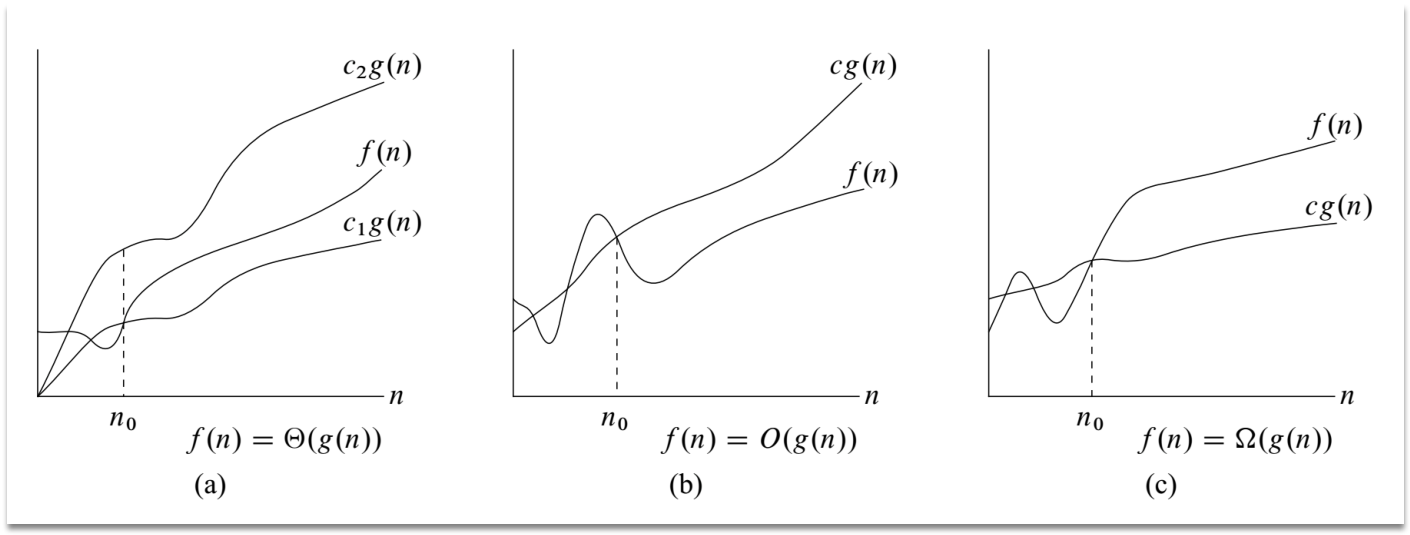
\includegraphics[scale=0.4]{images/asymptotic-notation.pdf}
  }
  \flushright{\itab}
  
\end{frame}

\begin{frame}{$\Theta$-notation}

  \begin{block}{Definition}
    \begin{itemize}
    \item For a given function $g(n)$, we define
      $\Theta(g(n))$ the set of functions:
    \end{itemize}
    
    \begin{small}
      \begin{multline*}
        \Theta(g(n)) = \{ f(n):\ there\ exist\ positive\ constants\ c_1,\ c_2,\ and\ n_0\ \\ such\ that\ 
                       0 \leq c_1g(n) \leq f(n) \leq c_2g(n)\ for\ all\ n \geq n0\}
      \end{multline*}
    \end{small}
  \end{block}

\end{frame}

\begin{frame}
  Example: $\frac{1}{2}n^2 - 3n \in \Theta(n^2)$ \pause

  \begin{itemize}
  \item We must determine positive constants $c_1$, $c_2$, and $n_0$,
    such that $c_1n^2 \leq \frac{1}{2}n^2 -3n \leq c2n^2$, for all $n \geq n_0$. \pause
  \item Possible solution for $n \geq 7$: \pause $c_1 \leq 1/14$ and $c_2 >= 1/2$.   
  \end{itemize} 
\end{frame}


\begin{frame}{$\mathcal{O}$-notation (asymptotic upper bound)}

  \begin{block}{Definition}
    \begin{itemize}
    \item For a given function $g(n)$, we define
      $\mathcal{O}(g(n))$ the set of functions:
    \end{itemize}
    
    \begin{small}
      \begin{multline*}
        \mathcal{O}(g(n)) = \{ f(n):\ there\ exist\ positive\ constants\ c,\ and\ n_0\ \\ such\ that\ 
                       0 \leq f(n) \leq cg(n)\ for\ all\ n \geq n0\}
      \end{multline*}
    \end{small}

    \begin{itemize}
      \item Note that $f(n) \in \Theta(g(n))$ implies $f(n) in \mathcal{O}(g(n))$  
    \end{itemize}
  \end{block}

\end{frame}

\begin{frame}{$\Omega$-notation (asymptotic lower bound)}

  \begin{block}{Definition}
    \begin{itemize}
    \item For a given function $g(n)$, we define
      $\Omega(g(n))$ the set of functions:
    \end{itemize}
    
    \begin{small}
      \begin{multline*}
        \Omega(g(n)) = \{ f(n):\ there\ exist\ positive\ constants\ c,\ and\ n_0\ \\ such\ that\ 
                       0 \leq c(g(n) \leq f(n)\ for\ all\ n \geq n0\}
      \end{multline*}
    \end{small}
  \end{block}

\end{frame}

\begin{frame}{$o$-notation (upper bound not asymptotically tight)}

  \begin{block}{Definition}
    \begin{itemize}
    \item For a given function $g(n)$, we define
      $\mathcal{o}(g(n))$ the set of functions:
    \end{itemize}
    
    \begin{small}
      \begin{multline*}
        o(g(n)) = \{ f(n):\ for\ any\ c > 0, there\ exists\ a\ positive\ constant\ n_0 > 0\ \\ such\ that\ 
                       0 \leq f(n) < cg(n) \ for\ all\ n \geq n0\}
      \end{multline*}
    \end{small}
  \end{block}

\end{frame}

\begin{frame}{$\omega$-notation (lower bound not asymptotically tight)}

  \begin{block}{Definition}
    \begin{itemize}
    \item For a given function $g(n)$, we define
      $\omega(g(n))$ the set of functions:
    \end{itemize}
    
    \begin{small}
      \begin{multline*}
        \omega(g(n)) = \{ f(n):\ for any c > 0, there\ exists\ a positive\ constant\ n_0 > 0\ \\ such\ that\ 
                       0 \leq cg(n) < f(n) \ for\ all\ n \geq n0\}
      \end{multline*}
    \end{small}
  \end{block}

\end{frame}


\begin{frame}{Running time of divide-and-conquer algorithms}

  \begin{itemize}
   \item Often involves a {\bf recurrence relation}. \pause
     The overall running time on a problem of size $n$ is described
     in terms of the running time on smaller inputs.

     \begin{itemize}
       \item Base case: when the input is small enough ($n \leq c$),
         the straightforward solution takes constant time ($T(n) = \Theta(1)$). \pause
         
       \item Recursive case: We split the problem into $a$ subproblems,
         each one having $\frac{1}{b}$ the size of the original input \pause(for MergeSort,
         $a = b = 2$). \pause Assuming we take $D(n)$ time to divide the problem into
         the subproblems and $C(n)$ to combine the solutions to the subproblems,
         we can derive a general solution for the running time of divide-and-conquer
         algorithms.
     \end{itemize}
  \end{itemize}
\end{frame}

\begin{frame}

  \begin{block}{General solution}
  \[ 
   T(n)= \left\{
   \begin{array}{ll}
     \Theta(1) & n \leq c, \\
     aT(n/b) + D(n) + C(n) & otherwise. \\
   \end{array} 
   \right. 
   \]
  \end{block}      

  \begin{itemize}
  \item There are three approaches for solving
    recurrence relations: the recursion-tree method,
    the substitution method, and the master method. 
  \end{itemize}
\end{frame}


\begin{frame}{Running time of MergeSort}

  Lets assume the input size is a power of 2 (1, 2, 4, 8, 16, 32, \ldots). pause
  Each divide step takes two subsequences of size $n/2$. \pause When we
  have $n > 1$ elements, we split the running time as follows:

  \begin{description}
   \item [Divide:] The divide step just computes the middle of the subarray (constant time).
     Therefore, $D(n) = \Theta(1)$.
   \item [Conquer:] The algorithm recursively solves two subproblems, each of size n/2.
     This contributes with $2T(n/2)$ to the running time.
     
   \item [Combine:] The merge procedure on $n$ elements takes time $\Theta(n)$, therefore
     $C(n) = \Theta(n)$
  \end{description}
\end{frame}

\begin{frame} 
  \[ 
   T(n)= \left\{
   \begin{array}{ll}
     \Theta(1) & if\ n = 1, \\
     2T(n/2) + \Theta(n) & if\ n > 1. \\
   \end{array} 
   \right. 
   \]
  
\end{frame}



\begin{frame}

  \[ 
   T(n)= \left\{
   \begin{array}{ll}
     c & if\ n = 1, \\
     2T(n/2) + cn & if\ n > 1. \\
   \end{array} 
   \right. 
   \]
  
\end{frame}

\begin{frame}

  \centering{
    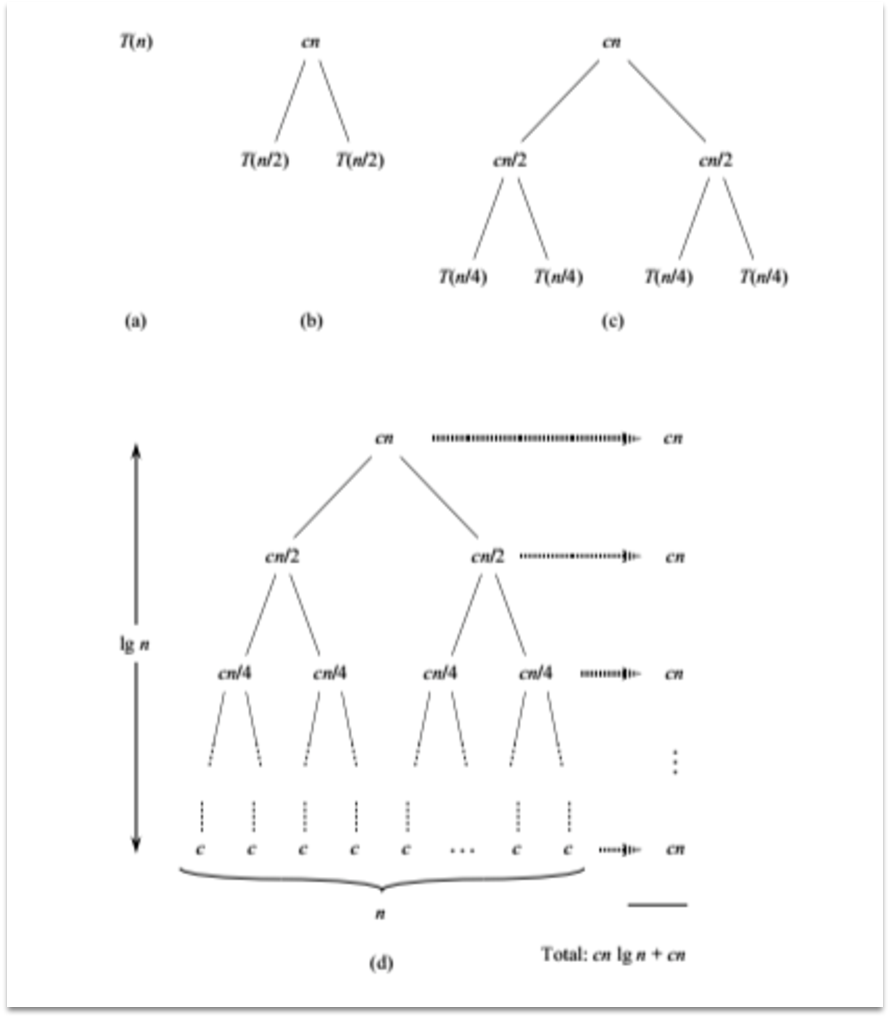
\includegraphics[scale=0.3]{images/recurrence-tree.pdf}
  }

  \flushright{\itab}
\end{frame}

\begin{frame}{The substitution method}
  \begin{block}{Two steps}
    \begin{itemize}
     \item Guess the form of the solution
     \item Proove that the solution works (using mathematical induction) 
    \end{itemize}
  \end{block}
\end{frame}

\begin{frame}{Example}

\begin{eqnarray*}
    T(n)  & = &  2T(\lfloor n/2 \rfloor) + n
\end{eqnarray*}  \pause

\begin{itemize}
\item Similar to the recurrence relation of the running time for MergeSort. \pause
  {\bf Guess}: the solution is $T(n) = \mathcal{O}(n log n)$. \pause So, we need to prove
  that $T(n) \leq c\ n\ log\ n$ for an appropriate choice of the const $c > 0$.
\end{itemize}
\end{frame}

\begin{frame}
\begin{itemize}
\item Lets assume this property holds for all positive $m < n$, in particular for
  $m = \lfloor n/2 \rfloor$. \pause This yields:

  \begin{eqnarray*}
    T(\lfloor n/2 \rfloor) & \leq & c \lfloor n/2 \rfloor log (\lfloor n/2 \rfloor)
  \end{eqnarray*}
      
\item  Substituting in the recurrence, we get:

  \begin{small}
\begin{eqnarray*}
  T(n) & \leq & 2  c \lfloor n/2 \rfloor log (\lfloor n/2 \rfloor) + n \\
       & \leq & c\ n\ log\ n/2 + n              \\
       & =    & c\ n\ log\ n - c\ n\ log\ 2 + n    \\
       & =    & c\ n\ log\ n - c\ n\ + n          \\
       & \leq & c\ n\ log\ n                    \\ 
 \end{eqnarray*}
  \end{small}
\end{itemize}
\end{frame}

\begin{frame}

\begin{itemize}
  \item It is also necessary to prove the base case (finding out a $n_0$ and $c$
    so that $T(n) \leq c\ n\ log\ n$). \pause T(1) does not hold for this example \pause, though for $n=2$ and
    $n=3$ it does.

  \item It is often necessary to elaborate the proof on some corner cases, by \emph{subtracting a lower-order term} or by
    \emph{changing variables}. The book covers these scenarios.     
\end{itemize}
\end{frame}


\begin{frame}{The (magic) master method}

  A ``cookbook'' for solving recurrences of the form:

  \begin{eqnarray*}
    T(n) & = & a\ T(n/b) + f(n)
  \end{eqnarray*}

   where $a \geq 1$, $b > 1$ and $f(n)$ is an asymptotivally positive function.

   \begin{block}{Three cases}
     \begin{scriptsize}
     \begin{itemize}
      \item if $f(n) = \mathcal{O}(n^{log_b a-\epsilon})$ for some constant $\epsilon > 0$\pause, then $T(n) = \Theta(n^{log_b a})$ \pause
      \item if $f(n) = \Theta(n^{log_b a})$\pause, then $T(n) = \Theta(n^{log_b a} log n)$\pause
      \item if $f(n) = \Omega(n^{log_b a + \epsilon})$ for some constant $\epsilon > 0$\pause, then $T(n) = \Theta(f(n))$ 
     \end{itemize}
     \end{scriptsize}
   \end{block}  
  
\end{frame}

\begin{frame}{Examples}

  \begin{itemize}
    \item $T(n) = 9T(n/3) + n$
    \item $T(n) = T(2n/3) + 1$
    \item $T(n) = 3T(n/4) + n\ log\ n$  
  \end{itemize}

\end{frame}


\section{Dynamic Programming}
\begin{frame}{Rod Cutting Problem}
  Given a rod of length $n$ inches and a table of prices $p_i$
  for $i = 1, 2, ..., n$, determine the maximum revenue $r_n$ obtainable
  by cutting up the rod and selling the pieces.

  \flushright{
    \scriptsize{(Cormen, Thomas H.. Introduction to Algorithms (p. 360). MIT Press).}}
\end{frame}

\begin{frame}
  \begin{tabular}{|c|cccc|cccccc|}\hline
    length $i$  & 1 & 2 & 3 & 4 & 5  & 6  & 7  & 8  & 9  & 10 \\ \hline
    price $p_i$ & 1 & 5 & 8 & 9 & 10 & 17 & 17 & 20 & 24 & 30 \\ \hline
  \end{tabular} \pause

  
  \centering{
    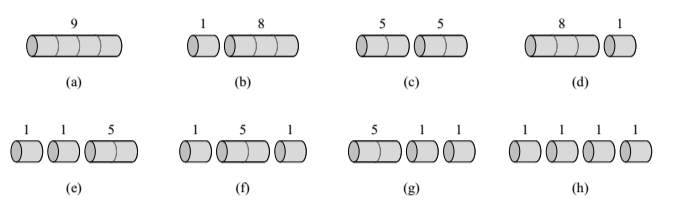
\includegraphics[scale=0.35]{images/rod-cutting}
  }

  \pause

  \begin{itemize}
   \item when $n = 4$, we have $2^{3}$ alternatives for cutting the rod. \pause
   \item $r_4  = max(p_4, r_3 + r_1, r_2 + r_2, r_1 + r_3)$ \pause
   \item $r_n  = max(p_n, r_1 + r_{n-1}, r_2 + r_{n-2}, ..., r_{n-1} + r1)$ \pause
   \item $r_n = max(p_i + r_{n-i})$, for $1 \geq i \geq n$       
  \end{itemize}
\end{frame}

\begin{frame}{Note}

  \begin{itemize}
  \item The {\color{blue}Rod Cutting} problem exhibits
    optimal substructure\pause: optimal solutions
    to a problem incorporate optimal solutions to related subproblems. 
  \end{itemize}
\end{frame}

\begin{frame}{Recursive top-down algorithm}

  \begin{block}{Recursive top-down strategy}
  \begin{algorithmic}
    \Procedure{CutRod}{p, n}
      \If{$n = 0$}
        \State {\bf return} $0$ 
      \EndIf
      \State $q = - \infty$
      \For{$i = 1 .. n$}
         \State $q = max(q, p[i] + CutRod(p, n-i))$ 
         \EndFor
      \State {\bf return} $q$   
    \EndProcedure
  \end{algorithmic}  
  \end{block}

\end{frame}

\begin{frame}[fragile]
  \begin{scriptsize}
  \begin{lstlisting}[language=Java]
public class RecursiveImplementation implements RodCutting {
  private static final int LESS_INFINITE = Integer.MIN_VALUE;

  @Override
  public int cutRod(int[] p, int n) {
    if(n == 0) {
      return 0;
    }
    int q = LESS_INFINITE;
    for(int i = 1; i <= n; i++) {
      q = max(q, p[i] + cutRod(p, n - i));
    }
    return q;
  }
}
  \end{lstlisting}
  \end{scriptsize}
\end{frame}

\begin{frame}
  \begin{itemize}
  \item Ineficient implementation: for $n = 10$, the algorithm
    calls \texttt{CutRod} 1024 times.
  \end{itemize}

  \pause
 
\vskip+1em
 \centering{   
  \begin{scriptsize}
  \begin{tabular}{cc} \toprule
     Value of $n$ & Number of calls \\ \midrule 
     0 & 512 \\
     1 & 256 \\
     2 & 128 \\
     3 & 64 \\
     4 & 32 \\
     5 & 16 \\
     6 & 8 \\
     7 & 4 \\
     8 & 2 \\
     9 & 1 \\
     10 & 1 \\ \bottomrule
  \end{tabular}
  \end{scriptsize}
  }

\end{frame}

\begin{frame}

  \begin{itemize}
  \item Optimization: keep precomputed values in a table (a process named {\color{blue}memoization}). \pause Here we use additional memory to save
    computation time (one of
  the components of dynamic programming).

  \end{itemize}
\end{frame}


\begin{frame}
  \begin{block}{Recursive top-down with memoization}
\begin{small}
    \begin{algorithmic}
      \Procedure{MemoizedCutRod}{p,n}
        \State $r = new Array[0..n]$
        \For{$i = 0 ... n$}
           \State $r[i] = - \infty$
        \EndFor
        \State $CutRodAux(p, n, r)$   
        \EndProcedure
    \end{algorithmic}
    \pause 
    \begin{algorithmic}
      \Procedure{CutRodAux}{p, n, r}
      \If{$r[n] \geq 0$}
        \State {\bf return} $r[n]$
      \EndIf
      \If{$n = 0$}
        \State $q = 0$ 
      \Else
        \State $q = - \infty$
        \For{$i = 1 .. n$}
          \State $q = max(q, p[i] + CutRodAux(p, n-i, r))$ 
        \EndFor
      \EndIf
      \State $r[n] = q$   
      \State {\bf return} $q$   
    \EndProcedure
  \end{algorithmic}  
 \end{small}
  \end{block}
\end{frame}


\begin{frame}
  \begin{block}{Bottom-up with memoization}
\begin{small}
    \begin{algorithmic}
      \Procedure{BottomUpCutRod}{p, n}
      \State $r = new Array[0..n]$
      \State $r[0] = 0$
      \For{$j = 1 ... n$}
       \State $q = - \infty$
       \For{$i = 1 ... j$}
          \State $q = max(q, p[i] + r[j-i]$
          \EndFor
          r[j] = q
       \EndFor
      \State {\bf return} $r[n]$   
    \EndProcedure
  \end{algorithmic}  
 \end{small}
  \end{block}
\end{frame}

\begin{frame}
  Most often, we are not only interested in computing the
  max revenue, but also find the places one must cut the rod to 
  lead to the max revenue. \pause There is a clever extension that adapts the
  bottom up solution to capture the first cut, and then
  reconstruct the entire solution. 
\end{frame}

\begin{frame}
  \begin{small}
    \begin{algorithmic}
      \Procedure{BottomUpCutRod}{p, n}
      \State $r = new Array[0..n]$
      \State $s = new Array[0..n]$

      \State $r[0] = 0$
      \For{$j = 1 ... n$}
       \State $q = - \infty$
       \For{$i = 1 ... j$}
       \If{$q  <  p[i] + r[j-i]$}
         \State $q = p[i] + r[j-i]$
         \State $s[j] = i$ 
       \EndIf
       \EndFor
          r[j] = q
       \EndFor
      \State {\bf return} $r[n], s$   
    \EndProcedure
    \end{algorithmic}
   \end{small} 

\end{frame}


\begin{frame}[fragile]{Longest Common Subsequence Problem}

  \begin{itemize}
  \item Application: compare (part of) the DNA of two (or more)
    different organisms. 
  \end{itemize}
  \pause

\begin{block}{Example} 
\begin{verbatim}
S1 = ACCGGTCGAGTGCGCGGAAGCCGGCCGAA
S2 = GTCGTTCGGAATGCCGTTGCTCTGTAAA
\end{verbatim}
\end{block}
\end{frame}

\begin{frame}
  
\begin{itemize}
\item The similarity between strands S1 and S2 might be
  computed by finding a common, third strand S3 in which the bases in S3 appear
  in each of S1 and S2. Note: the bases must appear  in the same order,
  but not necessarily at the same positions. The longest-common-subsequence is the
  longer common subsequence.

  \pause
  
\item Given two sequences $X = \langle A, B, C, B, D, A, B \rangle$ and
  $Y = \langle B, D, C, A, B, A \rangle$, the sequences $\langle B, C, A \rangle$ and
  $\langle B, C, B, A \rangle$ are common subsequences of both $X$ and $Y$\pause---the
  second one is one of the LCSs. 
\end{itemize}

\flushright{\scriptsize{(Cormen, Thomas H.. Introduction to Algorithms (p. 391). MIT Press.).}}

\end{frame}

\begin{frame}{Optimal Substructure of an LCS}

  Consider two sequences \seqb{X}{x_1, x_2, \ldots, x_m} and \seqb{Y}{y_1, y_2, \ldots, y_n} and
  let \seqb{Z}{z_1, z_2, \ldots, z_k} be any LCS of $X$ and $Y$. As such, one of the following
  situations might happen:

  \begin{small}
  \begin{enumerate}
    \item If $x_m = y_n$, then $z_k = x_m = y_n$ and $z_{k-1}$ is an LCS of $X_{m-1}$ and $Y_{n-1}$.
    \item If $x_m \neq y_n$ and $z_k \neq x_m$, then Z is an LCS of $X_{m-1}$ and $Y$.
    \item If $x_m \neq y_n$ and $z_k \neq x_m$, then Z is an LCS of $X$ and $Y_{n-1}$  
  \end{enumerate}
  \end{small}
\end{frame}

\begin{frame}{A recursive solution}

  \begin{itemize}
  \item Compute $c[i,j]$ as the length of an LCS of the sequences $X_i$ and $Y_j$.
    If either $i = 0$ or $j = 0$, one of the sequences has length $0$, and so the LCS
    has length $0$. \pause
  \end{itemize}
  
\[ 
c[i,j]= \left\{
\begin{array}{ll}
      0                         & if\ i = 0\ or\ j=0 \\ 
      c[i-1,j-1] + 1            & if\ i , j > 0\ and\ x_i = y_j \\   
      max(c[i, j-1], c[i-1,j])  & if\ i , j > 0\ and\ x_i \neq y_j
\end{array} 
\right. 
\]
  
\end{frame}  

\begin{frame}{A dynamic programming algorithm for LCS}

\begin{tiny}
    \begin{algorithmic}
      \Procedure{LCS}{X, Y}
      \State $m = X.length$
      \State $n = Y.length$
      \State $b = Array[1..m, 1..n]$
      \State $c = Array[1..m, 1..n]$
      \For{$i = 1 \ldots m$}
        \State $c[i, 0] = 0$
      \EndFor
      \For{$j = 1 \ldots n$}
        \State $c[0, j] = 0$
      \EndFor
      \For{$i = 1 \ldots m$}
        \For{$j = 1 \ldots n$}
          \If{$X[i] = Y[j]$}
            \State $c[i, j] = c[i-1, j-1] + 1$
            \State $b[i, j] = \nwarrow$
          \ElsIf {$c[i-1, j] \geq c[i, j-1]$}
            \State $c[i, j] = c[i-1, j]$
            \State $b[i, j] = \uparrow$
          \Else
            \State $c[i, j] = c[i, j-1]$
            \State $b[i, j] = \leftarrow$
         \EndIf  
       \EndFor
     \EndFor
      \State {\bf return} $c \ and\ b$    
    \EndProcedure
    \end{algorithmic}
   \end{tiny} 
\end{frame}


\begin{frame}
  \centering{
    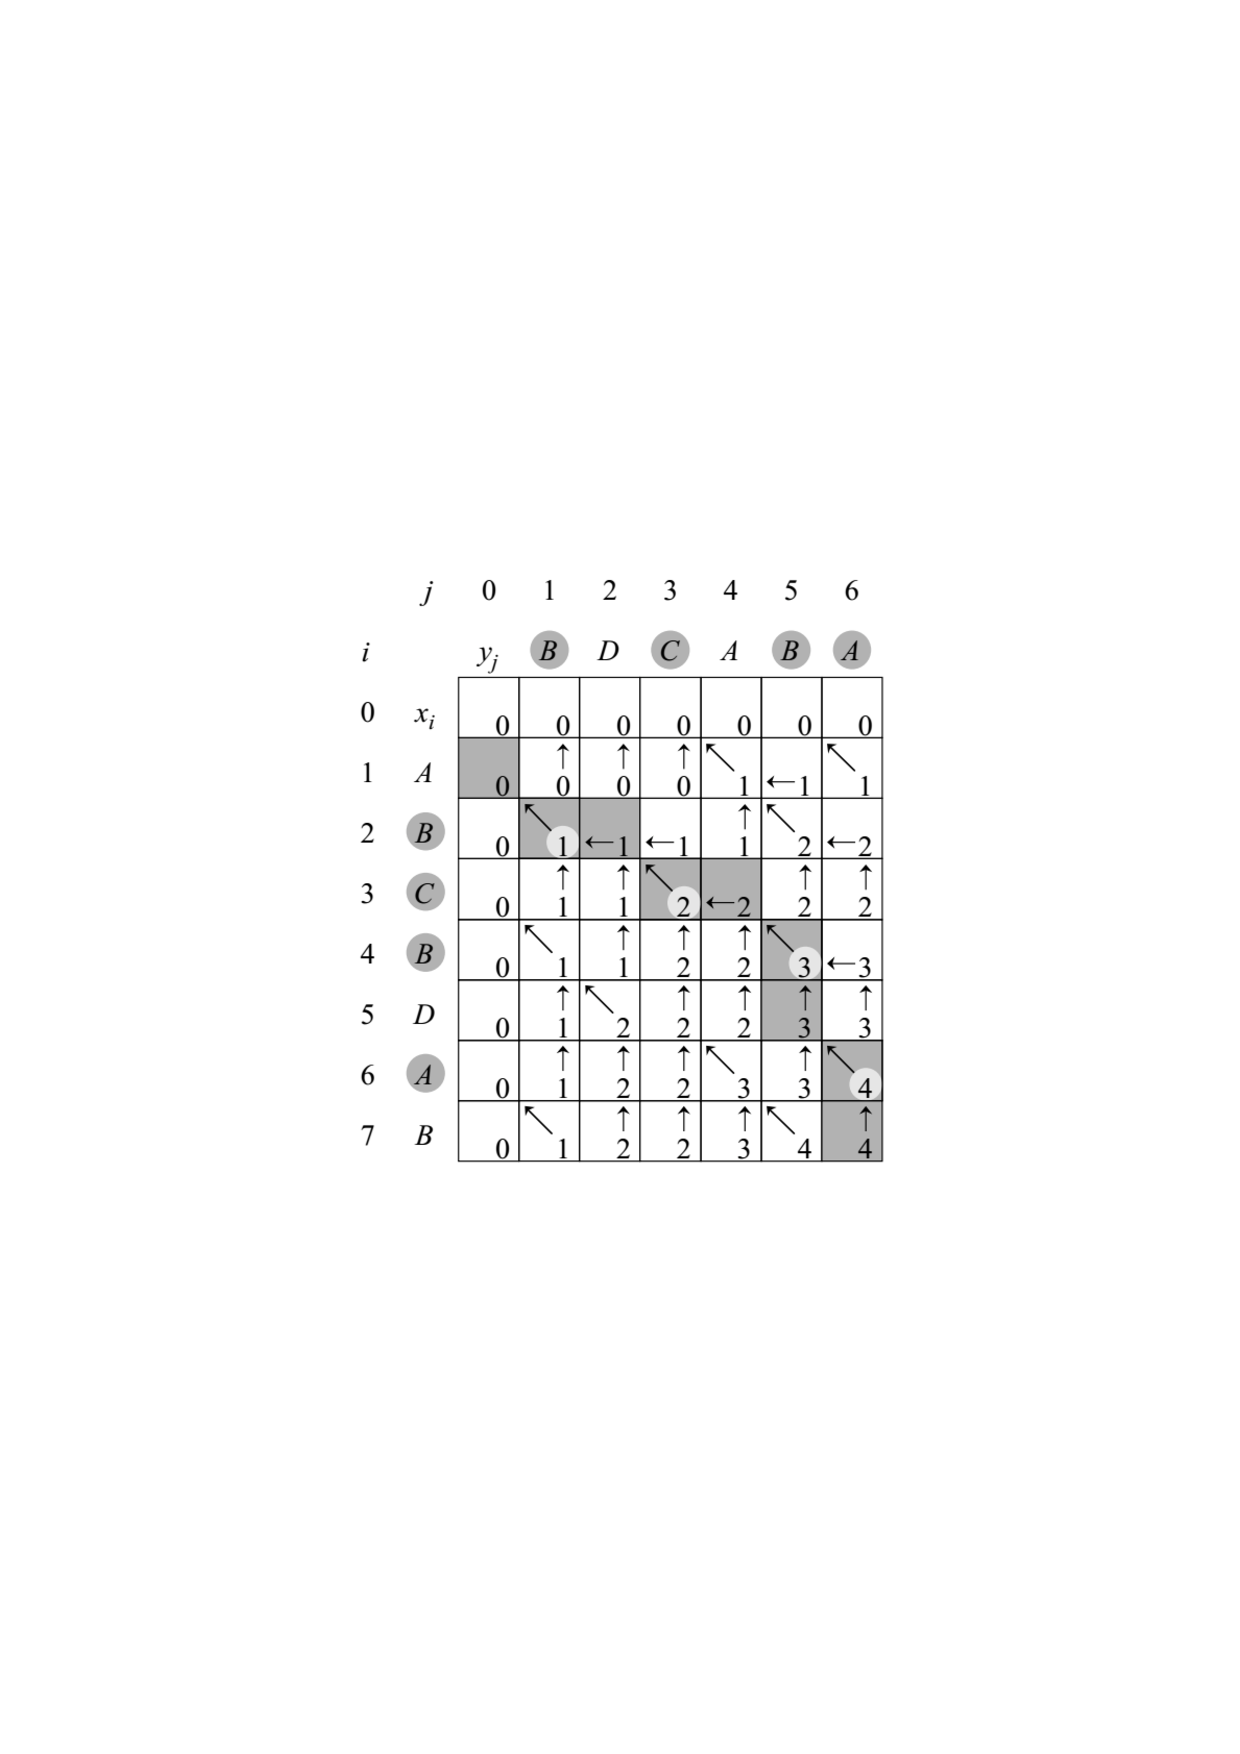
\includegraphics[trim=2cm 2cm 2cm 6cm,scale=0.5]{images/lcs.pdf}
    }
\end{frame}
\begin{frame}
\titlepage
\end{frame}

\section{Graph Algorithms}

	\begin{frame}
          \frametitle{Graphs}

          Pervasive data structure in Computer Science---an abstract
          representation in use to describe different domains, including
          trasport systems, electrical circuits, human interactions (social networks),
          computer networks, and software dependencies. \pause This class aims to
          discuss two concerns:   

          \vskip+1.5em

          \begin{itemize}
            \item graph representation 
            \item graph algorithms 
          \end{itemize}
        \end{frame}

\begin{frame}
\frametitle{Definition}

A graph $G$ is a pair $(V, E)$ where $V$ is an arbitrary
set and $E$ is a subset of $V^{(2)}$\pause---the set of all pairs of
elements in $V$.  The elements of $V$ are the {\color{blue}vertices} of the
graph, while the elements of $E$ are the {\color{blue}edges}
of the graph. 


\pause \vskip+1.5em
\begin{block}{Different flavors of graphs}

\begin{itemize}
\item directed graphs $\times$ undirected graphs
\item weighted graphs $\times$ unweighted graphs
\item ciclic graphs $\times$ aciclic graphs
\item \ldots
\end{itemize}
\end{block}
\end{frame}

\begin{frame}
\frametitle{Grapha representations}


\begin{itemize}
\item {\bf Adjacency-list:} compact representation recommended for
  {\color{blue}sparse graphs}  (where $|E|$ is smaller than 
  $|V|^{2}$). \pause 

\item {\bf Adjacency-matrix:} recommended for dense graphs or when we
  need to frequently search if an edge $(v_1, v_2)$ exists.   
\end{itemize}

\end{frame}

\begin{frame}
\frametitle{Samples (Fonte: Introduction to Algorithms)}
\centering{

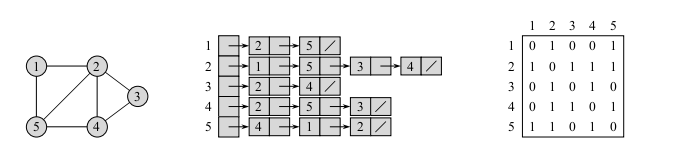
\includegraphics[scale=0.5]{images/undirected01.png}

\pause 

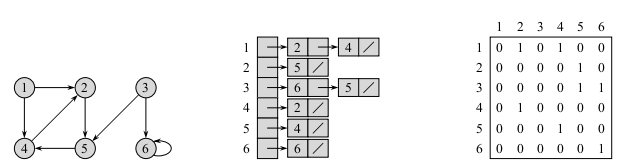
\includegraphics[scale=0.5]{images/directed01.png}	
}

\end{frame}


\begin{frame}
  \frametitle{Graph Algorithms}

  \begin{itemize}
   \item Search: Breadth-first search and Depth-first Search
   \item Single source shortest paths: Belkman-Ford and Dijkstra algorithms
   \item {\color{blue}Minimum Spanning Trees}
   \item {\color{blue}All-pairs shortest paths}  
  \end{itemize}
\end{frame}

\begin{frame}{Minimum Spanning Trees}

  Given a connected, weighted, and undirected graph $G = (V, E)$, we wish to
  find an acyclic subset $T \subseteq E$ that connects all of the vertices
  and whose {\color{blue}total} weight is minimized. \pause Since $T$ is acyclic and
  connects all of the vertices, it must form a (spanning) tree. 

  \pause \vskip+1.5em

  \centering{
    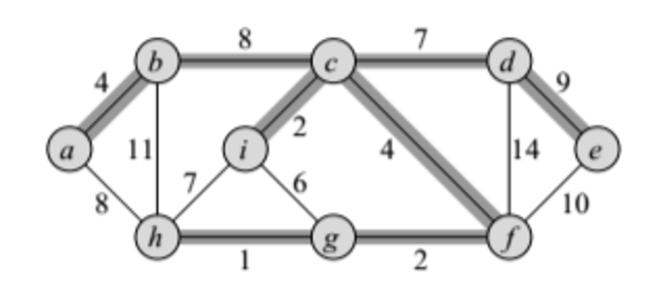
\includegraphics[scale=0.5]{images/st}
  }
\end{frame}


\begin{frame}

  The book presents an interesting description of the algortihms for
  Minimum Spanning Trees: a generic method for growing minimum spanning trees
  and two implementations of the algorithm (Kruskal's algorithm and Prim's algorithm).

  \pause \vskip+1.5em

  \begin{block}{Generic Method}
  \begin{algorithmic}
    \Procedure{Generic-MST}{G, w}
     \State $A = \emptyset$                 
     \While{$\text{A does not form a spanning tree}$}        
       \State $\text{find an edge (u, v) that is safe for A}$
       \State $A = A \cup \{(u, v)\}$
     \EndWhile
     \State {\bf return} $A$
    \EndProcedure
  \end{algorithmic}
  \end{block}

  \pause

  \begin{itemize}
    \item The challenge is to find out a {\color{blue}safe edge (u, v)}. 
  \end{itemize}
\end{frame}

\begin{frame}{Definitions}

  \begin{itemize}
   \item A {\color{blue}$cut(S, V-S)$} of an undirected graph $G = (V, E)$ is a partition of $V$. \pause 

   \item An {\color{blue}edge $(u, v) \in E$ crosses} a $cut(S, V-S)$ if one of its endpoints is in $S$ and
     the other is in $V-S$. \pause

   \item A {\color{blue}cut respects} a set A of edges if no edge in A crosses the cut. \pause
     
   \item An edge is a {\color{blue}light edge crossing} a cut if its weight is the minimum of any
     edge crossing the cut.  
  \end{itemize}
\end{frame}

\begin{frame}
  \begin{block}{Theorem}
    Given:
    \begin{itemize}
      \item $G = (V, E)$ is a connected, undirected graph
      \item $w : E \rightarrow R$ is a weighted function.
      \item $A$ is a subset of $E$ (included in some minimum spanning subtree for $G$)
      \item $(S, V-S)$ is any cut of $G$ that respects $A$
      \item $(u, v)$ is a light edge crossing $(S, V-S)$
    \end{itemize}
    then, edge $(u, v)$ is safe for $A$. 
  \end{block}

  Both algorithm implementations relie on this theorem. 
\end{frame}

\begin{frame}
  In the Kruskal's algorithm, the set $A$ is a {\color{blue}forest}
  whose vertices are all those of the given graph. The safe edge
  added to $A$ is allways a lest-weight edge in the graph that
  connects two distinct trees in the forest. \pause The book
  shows an implementation that benefits from the Disjoint Set
  data structure, whose interface contains three operations:
  \texttt{makeSet}, \texttt{findSet}, and \texttt{union}. 
\end{frame}

\begin{frame}
  \begin{small}
  \begin{algorithmic}
    \Procedure{MST-Kruskal}{G, w}
    \For{$\text{each vertex v } \in G.V$}
      \State $makeSet(v)$
    \EndFor
    \State $lst = \text{sort the edges of G.E into nondecreasing order by weight w}$
    \For{$(u, v) \rightarrow lst$}
      \If{$findSet(u) \neq findSet(v)$}
       \State $A = A \cup \{(u, v)\}$
       \State $union(u, v)$
      \EndIf 
    \EndFor
    \State {\bf return} $A$  
    \EndProcedure
  \end{algorithmic}
  \end{small}
\end{frame}

\begin{frame}{TODO}

  Study and implement the Prim's algorithm for
  computing minimum spanning trees. 
 
\end{frame}


\end{document}





